% questions.tex —— 2008 年·全国大纲卷Ⅰ·文科 · 题目内容片段（无答案）
% 由 tools/generate_projects.py 依来源总账自 2008/2008_数学真题_全国1文_试题.md 生成，勿手改（改源 MD 后重跑）


\gkpart{数学}

\begin{gktip}
\textbf{来源说明}：本题面依据固定源 PDF 两页 A3 题面逐题转录，原卷印刷页码 435–436。固定源不附答案，答案和解析均由本库独立复算。

\textbf{图形说明}：第 2、18 题的原卷图形关系重绘为 TikZ/PGFPlots 矢量图。图形标记所指的 PNG 不随仓库保存。
\end{gktip}

\gkpart{一、选择题}

\begin{question}
\gkti{1}函数 $y=\sqrt{1-x}+\sqrt{x}$ 的定义域为\mbox{（　　）}

（A）$\{x\mid x\leqslant1\}$\\
（B）$\{x\mid x\geqslant0\}$\\
（C）$\{x\mid x\geqslant1\text{ \text{或} }x\leqslant0\}$\\
（D）$\{x\mid0\leqslant x\leqslant1\}$

\Needspace{0.4\textheight}
\end{question}
\begin{question}
\gkti{2}汽车经过启动、加速行驶、匀速行驶、减速行驶之后停车，若把这一过程中汽车的行驶路程 $s$ 看作时间 $t$ 的函数，其图象可能是\mbox{（　　）}
\nopagebreak[4]
\begin{center}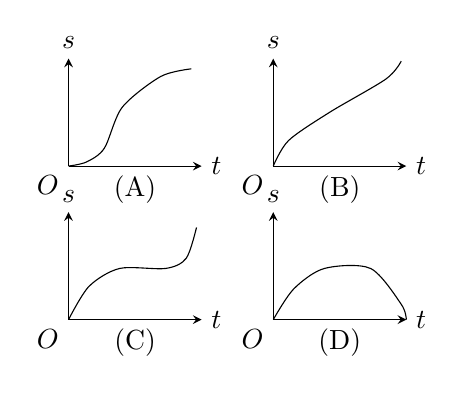
\begin{tikzpicture}[>=stealth,scale=.65]
\foreach \x/\y/\lab in {0/0/A,4/0/B,0/-3/C,4/-3/D}{
  \begin{scope}[shift={(\x,\y)}]
    \draw[->] (0,0)--(2.6,0) node[right] {$t$};
    \draw[->] (0,0)--(0,2.1) node[above] {$s$};
    \node[below left] at (0,0) {$O$};
    \node at (1.3,-.45) {(\lab)};
  \end{scope}
}
\draw plot[smooth] coordinates {(0,0) (.35,.08) (.7,.35) (1.05,1.15) (1.8,1.75) (2.4,1.9)};
\draw[shift={(4,0)}] plot[smooth] coordinates {(0,0) (.3,.5) (1.1,1.05) (2.2,1.7) (2.5,2.05)};
\draw[shift={(0,-3)}] plot[smooth] coordinates {(0,0) (.4,.65) (1.0,1.0) (1.9,1.0) (2.3,1.2) (2.5,1.8)};
\draw[shift={(4,-3)}] plot[smooth] coordinates {(0,0) (.4,.6) (1.0,1.0) (1.9,1.0) (2.5,.3) (2.6,0)};
\end{tikzpicture}
\end{center}
\nopagebreak[4]
（A）图 A\\
（B）图 B\\
（C）图 C\\
（D）图 D

\end{question}
\begin{question}
\gkti{3}$\left(1+\dfrac{x}{2}\right)^5$ 的展开式中 $x^2$ 的系数为\mbox{（　　）}

（A）$10$\quad（B）$5$\quad（C）$\dfrac52$\quad（D）$1$

\end{question}
\begin{question}
\gkti{4}曲线 $y=x^3-2x+4$ 在点 $(1,3)$ 处的切线的倾斜角为\mbox{（　　）}

（A）$30^\circ$\quad（B）$45^\circ$\quad（C）$60^\circ$\quad（D）$120^\circ$

\end{question}
\begin{question}
\gkti{5}在 $\triangle ABC$ 中，$\overrightarrow{AB}=\boldsymbol c$，$\overrightarrow{AC}=\boldsymbol b$。若点 $D$ 满足 $\overrightarrow{BD}=2\overrightarrow{DC}$，则 $\overrightarrow{AD}=$\mbox{（　　）}

（A）$\dfrac23\boldsymbol b+\dfrac13\boldsymbol c$\quad（B）$\dfrac53\boldsymbol c-\dfrac23\boldsymbol b$\quad（C）$\dfrac23\boldsymbol b-\dfrac13\boldsymbol c$\quad（D）$\dfrac13\boldsymbol b+\dfrac23\boldsymbol c$

\end{question}
\begin{question}
\gkti{6}$y=(\sin x-\cos x)^2-1$ 是\mbox{（　　）}

（A）最小正周期为 $2\pi$ 的偶函数\\
（B）最小正周期为 $2\pi$ 的奇函数\\
（C）最小正周期为 $\pi$ 的偶函数\\
（D）最小正周期为 $\pi$ 的奇函数

\end{question}
\begin{question}
\gkti{7}已知等比数列 $\{a_n\}$ 满足 $a_1+a_2=3$，$a_2+a_3=6$，则 $a_7=$\mbox{（　　）}

（A）$64$\quad（B）$81$\quad（C）$128$\quad（D）$243$

\end{question}
\begin{question}
\gkti{8}若函数 $y=f(x)$ 的图象与函数 $y=\ln\sqrt{x}+1$ 的图象关于直线 $y=x$ 对称，则 $f(x)=$\mbox{（　　）}

（A）$e^{2x-2}$\quad（B）$e^{2x}$\quad（C）$e^{2x+1}$\quad（D）$e^{2x+2}$

\end{question}
\begin{question}
\gkti{9}为得到函数 $y=\cos\left(x+\dfrac\pi3\right)$ 的图象，只需将函数 $y=\sin x$ 的图象\mbox{（　　）}

（A）向左平移 $\dfrac\pi6$ 个长度单位\\
（B）向右平移 $\dfrac\pi6$ 个长度单位\\
（C）向左平移 $\dfrac{5\pi}6$ 个长度单位\\
（D）向右平移 $\dfrac{5\pi}6$ 个长度单位

\end{question}
\begin{question}
\gkti{10}若直线 $\dfrac{x}{a}+\dfrac{y}{b}=1$ 与圆 $x^2+y^2=1$ 有公共点，则\mbox{（　　）}

（A）$a^2+b^2\leqslant1$\quad（B）$a^2+b^2\geqslant1$\quad（C）$\dfrac1{a^2}+\dfrac1{b^2}\leqslant1$\quad（D）$\dfrac1{a^2}+\dfrac1{b^2}\geqslant1$

\end{question}
\begin{question}
\gkti{11}已知三棱柱 $ABC-A_1B_1C_1$ 的侧棱与底面边长都相等，$A_1$ 在底面 $ABC$ 内的射影为 $\triangle ABC$ 的中心，则 $AB_1$ 与底面 $ABC$ 所成角的正弦值等于\mbox{（　　）}

（A）$\dfrac13$\quad（B）$\dfrac{\sqrt2}{3}$\quad（C）$\dfrac{\sqrt3}{3}$\quad（D）$\dfrac23$

\end{question}
\begin{question}
\gkti{12}将 $1,2,3$ 填入 $3\times3$ 的方格中，要求每行、每列都没有重复数字，下面是一种填法，则不同的填写方法共有\mbox{（　　）}

\nopagebreak[4]
\[
\begin{matrix}1&2&3\\3&1&2\\2&3&1\end{matrix}
\]

（A）$6$ 种\quad（B）$12$ 种\quad（C）$24$ 种\quad（D）$48$ 种

\end{question}
\gkpart{二、填空题}

\begin{question}
\gkti{13}若 $x,y$ 满足约束条件

\nopagebreak[4]
\[
\begin{cases}
x+y\geqslant0,\\
x-y+3\geqslant0,\\
0\leqslant x\leqslant3,
\end{cases}
\]

则 $z=2x-y$ 的最大值为\gkblank{}。

\end{question}
\begin{question}
\gkti{14}已知抛物线 $y=ax^2-1$ 的焦点是坐标原点，则以抛物线与两坐标轴的三个交点为顶点的三角形面积为\gkblank{}。

\end{question}
\begin{question}
\gkti{15}在 $\triangle ABC$ 中，$\angle A=90^\circ$，$\tan B=\dfrac34$。若以 $A\text{、}B$ 为焦点的椭圆经过点 $C$，则该椭圆的离心率 $e=$\gkblank{}。

\end{question}
\begin{question}
\gkti{16}已知菱形 $ABCD$ 中，$AB=2$，$\angle A=120^\circ$，沿对角线 $BD$ 将 $\triangle ABD$ 折起，使二面角 $A-BD-C$ 为 $120^\circ$，则点 $A$ 到 $\triangle BCD$ 所在平面的距离等于\gkblank{}。

\end{question}
\gkpart{三、解答题}

\begin{question}
\gkti{17}设 $\triangle ABC$ 的内角 $A,B,C$ 所对的边长分别为 $a,b,c$，且 $a\cos B=3$，$b\sin A=4$。

（1） 求边长 $a$；

（2） 若 $\triangle ABC$ 的面积 $S=10$，求 $\triangle ABC$ 的周长 $l$。

\Needspace{0.4\textheight}
\end{question}
\begin{question}
\gkti{18}四棱锥 $A-BCDE$ 中，底面 $BCDE$ 为矩形，侧面 $ABC\perp$ 底面 $BCDE$，$BC=2$，$CD=\sqrt2$，$AB=AC$。
\nopagebreak[4]
\begin{center}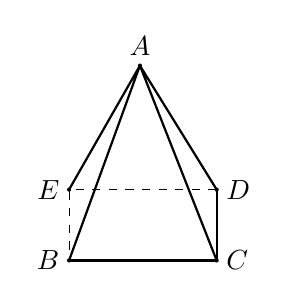
\begin{tikzpicture}[scale=.75,>=stealth]
\coordinate (B) at (0,0); \coordinate (C) at (2.5,0);
\coordinate (D) at (2.5,1.2); \coordinate (E) at (0,1.2);
\coordinate (A) at (1.2,3.3);
\draw[thick] (B)--(C)--(D); \draw[dashed] (D)--(E)--(B);
\draw[thick] (A)--(B) (A)--(C) (A)--(D) (A)--(E);
\draw[dashed] (A)--(D);
\fill (A) circle (1pt) node[above] {$A$};
\fill (B) circle (1pt) node[left] {$B$};
\fill (C) circle (1pt) node[right] {$C$};
\fill (D) circle (1pt) node[right] {$D$};
\fill (E) circle (1pt) node[left] {$E$};
\end{tikzpicture}
\end{center}
\nopagebreak[4]
（1） 证明：$AD\perp CE$；

（2） 设侧面 $ABC$ 为等边三角形，求二面角 $C-AD-E$ 的大小。

\end{question}
\begin{question}
\gkti{19}在数列 $\{a_n\}$ 中，$a_1=1$，$a_{n+1}=2a_n+2^n$。

（1） 设 $b_n=\dfrac{a_n}{2^{n-1}}$，证明：数列 $\{b_n\}$ 是等差数列；

（2） 求数列 $\{a_n\}$ 的前 $n$ 项和 $S_n$。

\end{question}
\begin{question}
\gkti{20}已知 $5$ 只动物中有 $1$ 只患有某种疾病，需要通过化验血液来确定患病的动物。血液化验结果呈阳性的即为患病动物，呈阴性即没患病。下面是两种化验方案：

方案甲：逐个化验，直到能确定患病动物为止。

方案乙：先任取 $3$ 只，将它们的血液混在一起化验。若结果呈阳性则表明患病动物为这 $3$ 只中的 $1$ 只，然后再逐个化验，直到能确定患病动物为止；若结果呈阴性则在另外 $2$ 只中任取 $1$ 只化验。

求依方案甲所需化验次数不少于依方案乙所需化验次数的概率。

\end{question}
\begin{question}
\gkti{21}已知函数 $f(x)=x^3+ax^2+x+1$，$a\in\mathbb R$。

（1） 讨论函数 $f(x)$ 的单调区间；

（2） 设函数 $f(x)$ 在区间 $\left(-\dfrac23,-\dfrac13\right)$ 内是减函数，求 $a$ 的取值范围。

\end{question}
\begin{question}
\gkti{22}双曲线的中心为原点 $O$，焦点在 $x$ 轴上，两条渐近线分别为 $l_1,l_2$，经过右焦点 $F$ 垂直于 $l_1$ 的直线分别交 $l_1,l_2$ 于 $A,B$ 两点。已知 $\overrightarrow{OA}$、$\overrightarrow{AB}$、$\overrightarrow{OB}$ 成等差数列，且 $\overrightarrow{BF}$ 与 $\overrightarrow{FA}$ 同向。

（1） 求双曲线的离心率；

（2） 设 $AB$ 被双曲线所截得的线段的长为 $4$，求双曲线的方程。

\end{question}